\documentclass{article}

\usepackage[utf8x]{inputenc}
\usepackage[english,russian]{babel}
\usepackage{graphicx}
\usepackage{amsmath}
\usepackage{amssymb}
\usepackage{extarrows}
\usepackage{vmargin}
\usepackage{MnSymbol}
\setpapersize{A4}
\setmarginsrb{2cm}{2cm}{2cm}{2cm}{0pt}{0mm}{0pt}{13mm}
%\usepackage{cmap}

\newtheorem{theorem}{Теорема}


\begin{document}

\centerline{\large Курс лекция для магистров ВМК МГУ}
\centerline {\textbf{\LARGE Обратные задачи математической физики}}
\centerline {Затехал Строков Вениамин 2025}

\vspace{0.4cm}

\centerline{\LARGE 	Лекция 5. Некорректные и обратные задачи распространения волн}
\centerline{\LARGE 	в трещеноватой среде}

\vspace{0.5cm}

\subsection*{Волновое уравнение с комплексной скоростью}


\vspace{0.2cm}
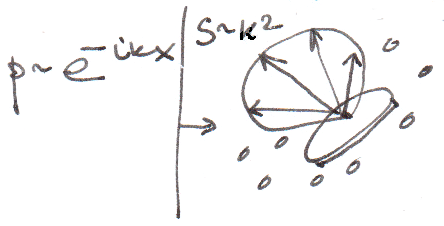
\includegraphics[scale=0.75]{pic5_1.png}
\vspace{0.2cm}


На трещинах происходит рэлеевское рассеяние:
$$\begin{cases}
    s_{tt} &= a^2 s_{xx} - 2 \nu p_{tt}, \quad 0 < \nu \ll 1, \\
    p_{tt} &= a^2 p_{xx} + 2 \nu s_{tt}, \quad s \sim \sqrt{
u}.
\end{cases}$$

Обозначим $\mathbf{w} = p + i s$, тогда
\begin{equation*}
    \mathbf{w}_{tt} = a^2 (1 - i \nu)^2 \mathbf{w}_{xx} \quad \text{(с точностью до } \nu^2 \text{)}.
\end{equation*}

Рассмотрим частное решение в виде
\begin{equation*}
    \mathbf{w} = A(k) e^{i(\omega t - kx)}.
\end{equation*}

Подставляя в уравнение, получаем условие разрешимости

\begin{equation*}
    \begin{vmatrix}
        \omega^2 - a^2 k^2 & 2\nu \omega^2 \\
        -2 \nu \omega^2 & \omega^2 - a^2 k^2
    \end{vmatrix}
    A(k) = 0 \quad \Leftrightarrow \quad \det = 0.
\end{equation*}

Решая характеристическое уравнение,
\begin{equation}
    (\omega^2 - a^2 k^2)^2 + 4 \nu^2 \omega^4 = 0,
    \label{characteristic}
\end{equation}

получаем
\begin{equation*}
    \omega^2 - a^2 k^2 = \pm 2 i \nu \omega^2.
\end{equation*}

Выразим $a(\omega)$:
\begin{equation*}
    ak(\omega) = \pm (1 \pm 2 i \nu) \omega.
\end{equation*}

То есть уравнение (\ref{characteristic}) имеет 4 корня (с точностью до $O(\nu^2)$).

Таким образом, записываем частные решения:
\begin{equation*}
    \mathbf{w}(x,t) = A(k) e^{\pm i(\omega t \pm \omega x/a)} e^{\pm \nu \omega t}.
\end{equation*}

%Следовательно, импульс убывает при $t, x \to \pm\infty$.
Следовательно, есть решения $\to \infty$ при $t, x \to \pm\infty$.



Рассмотрим следующую начальную задачу

Рассмотрим задачу Коши:
\begin{equation}
    \mathbf{w}_{tt} = a^2 (1 - i \nu)^2 \mathbf{w}_{xx}, \quad -\infty < x < \infty, \quad t > 0,
\end{equation}

с начальными условиями
\begin{equation*}
    \mathbf{w}(x,0) = \mathbf{w}_0(x), \quad -\infty < x < \infty,
\end{equation*}

где $\mathbf{w}_0(x) \in L^1(\mathbb{R})$.

Решением назовем $\mathbf{w} = p + i s$, где $\mathbf{w} \in W^1_2(\mathbb{R})$, ограниченное при $t > 0$.

Используем преобразование Фурье по переменной $x$:
\begin{equation*}
    \Phi_{x \to k} \mathbf{w} = U(k,t), \quad x \to k.
\end{equation*}

Рассматриваем уравнение:
\begin{equation*}
    U_{tt} + a^2 (1 - i\nu)^2 k^2 U(k,t) = 0.
\end{equation*}

Решение имеет вид:
\begin{equation*}
    U(k,t) =
	\begin{cases}
     U_0^+(k) e^{i a k t + \nu a k t} + U_0^-(k) e^{-i a k t - \nu a k t}, & k \in \mathbb{R} \setminus 0;\\
     U_0 + U_1 t,  & k =0.
     \end{cases}
\end{equation*}

Выделим ограниченное решение при $t \to \infty$:
\begin{equation*}
    U(k,t) =
	\begin{cases}
      U_0^-(k) e^{-i a k t - \nu a k t}, & k \geqslant 0;\\
      U_0^+(k) e^{i a k t + \nu a k t},  & k <0.
     \end{cases}
     = U_0(k) e^{-i a |k| t - \nu a |k| t}
\end{equation*}

где
\begin{equation*}
    U_0(k) = \Phi_{x \to k} \mathbf{w}_0(x).
\end{equation*}

Условие для $\mathbf{w}_t(x,0)$ не ставим. Таким образом это задача Дирихле.

\textbf{Замечание}: Можно показать, что общее решение исходного уравнения имеет вид "комплексных бегущих" волн, то есть:
\begin{equation*}
\mathbf{w}(x,t) = f(x-a(1+i\nu)t) + g(x + a(1+i\nu)t),
\end{equation*}

однако решение начальной задачи, не ограниченное (за исключением $\mathbf{w}_0(x) = const$), представимо в виде
\begin{equation*}
\mathbf{w}(x,t) = \dfrac{1}{2}(\mathbf{w}_0 (x-a(1-i\nu)t) + \mathbf{w}_0(x + a(1-i\nu)t),
\end{equation*}

где $\mathbf{w}_0$ аналитическая при $\forall x,t$ 


Пусть теперь $\mathbf{w}_0(x) \in L_1(\mathbb{R}) \cap C^1(\mathbb{R})$. Запишем интегральное представление решения:
\begin{equation*}
    \mathbf{w}(x,t) = \int_{-\infty}^{\infty} \mathbf{w}_0(\xi) \mathcal{F}(x-\xi,t) d\xi,
\end{equation*}

где ядро
$$
\mathcal{F}(x,t) = \frac{1}{2\pi} \int_{-\infty}^{\infty} e^{i k x} e^{-i a |k|t - \nu a |k|t} d k 
= \left\{ e^{ikx} = cos(|k|x)+ i sin(|k|x) \right\} = 
$$$$
= \dfrac{1}{4 \pi} \int_{-\infty}^{\infty} (e^{i|k|x} + e^{-i|k|x}) e^{-ia|k|t - \nu a |k|t} dk  
= \left\{ \int_{-\infty}^{\infty} (e^{i \alpha |k| - \beta |k|} dk =
\dfrac{2}{\beta - i \alpha} \right\} =
$$$$
= \frac{1}{2\pi} \left( \frac{1}{\nu a t - i x + i a t} + \frac{1}{\nu a t + i x + i a t} \right) 
= \frac{1}{2\pi} \left( \frac{\nu a t + i x - i a t}{(x - a t)^2 + (\nu a t)^2} + 
\frac{\nu a t - i x - i a t}{(x + a t)^2 + (\nu a t)^2} \right).
$$ % стоит перепроверить последний переход

Таким образом, имеем решение, ограниченное при $t \to \infty$
\begin{equation*}
    p(x,t) = \frac{1}{2\pi} \int_{-\infty}^{\infty} \left( \frac{\nu a t}{(x - \xi - a t)^2 + (\nu a t)^2} + \frac{\nu a t}{(x - \xi + a t)^2 + (\nu a t)^2} \right) \varphi(\xi) d\xi 
\end{equation*}

\begin{equation*}
	- \frac{1}{2\pi} \int_{-\infty}^{\infty} \left( \frac{x - \xi - a t}{(x - \xi - a t)^2 + (\nu a t)^2} - \frac{x - \xi + a t}{(x - \xi + a t)^2 + (\nu a t)^2} \right) \psi(\xi) d\xi
\end{equation*}

\begin{equation*}
    S(x,t) = \frac{1}{2\pi} \int_{-\infty}^{\infty} \left( \frac{\nu a t}{(x - \xi - a t)^2 + (\nu a t)^2} + \frac{\nu a t}{(x - \xi + a t)^2 + (\nu a t)^2} \right) \psi(\xi) d\xi 
\end{equation*}

\begin{equation*}
    + \frac{1}{2\pi} \int_{-\infty}^{\infty} \left( \frac{x - \xi - a t}{(x - \xi - a t)^2 + (\nu a t)^2} - \frac{x - \xi + a t}{(x - \xi + a t)^2 + (\nu a t)^2} \right) \varphi(\xi) d\xi
\end{equation*}

Доказывается, что построенное решение единственно.


\subsection*{Обратная задача рассеяния на полупрямой}

Рассмотрим уравнение для рассеяния поля
$$
\text{ПЗ1}
\begin{cases}
s_{tt} = a^2 s_{xx} + \nu(x) p_{tt}^0(x,t),& x > 0, t > 0;\\
s(x,0) = s_t(x,0) = 0, & x \geqslant 0;\\
s_x(0,t) = 0, & t \geqslant 0;
\end{cases}
$$

где $p^0(x,t)$ - решение начально-краевой задачи (линеаризованной по $\nu$)

$$
\text{ПЗ0}
\begin{cases}
	p_{tt} = a^2 p_{xx},& x > 0, t > 0;\\
	p(x,0) = p_t(x,0) = 0, & x \geqslant 0;\\
	ap_x(0,t) = -\varphi(t), & t \geqslant 0;
\end{cases}
$$

где $\varphi(\xi) = 0, \xi \leqslant 0$, $\varphi \in C^1[0, \infty)$. Следовательно $p^0(x,t) = \varphi(t-x/a)$.


\vspace{0.2cm}
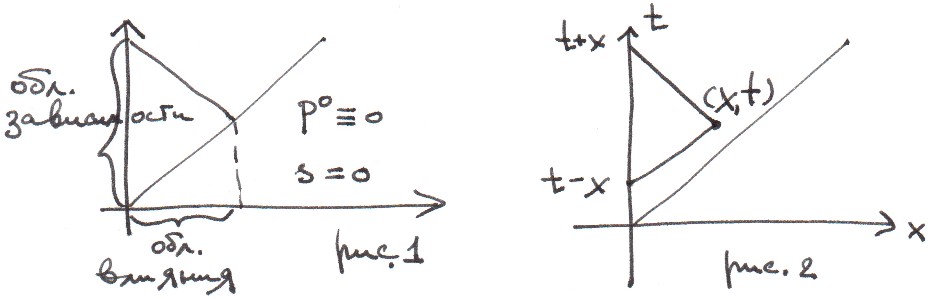
\includegraphics[scale=0.55]{pic5_2.png}
\vspace{0.2cm}


ОЗ: Дано $\varphi$, $S(0,t) = f(t), 0 \leqslant t \leqslant T$. Требуется найти $\nu(x), x \in [0,T]$.

Из формулы Даламбера имеем
\begin{equation*}
	s(x,t) = \dfrac{f(t + x/a) + f(t - x/a)}{2} +
	\dfrac{1}{2a} \int_0^x \int_{t-(x-\xi)/a}^{t+(x-\xi)/a} \nu(\xi) \varphi'(\tau - \frac{\xi}{a}) d\tau d\xi =
\end{equation*}
\begin{equation*}
	= \dfrac{f(t + x/a) + f(t - x/a)}{2} +
	\dfrac{1}{2a} \int_0^x \nu(\xi) [ \varphi(t - \frac{x-2\xi}{a}) - \varphi(t - \frac{x}{a})] d\xi.
\end{equation*}

Используя условие (при $x = at$) $S(x,x/a) = 0$ получим 
\begin{equation*}
	f(2t) + \dfrac{1}{a} \int_0^{at} \nu(\xi) [\varphi(2(t - \frac{\xi}{a})) - \varphi(0)] d\xi = 0,
	 \hspace{0.5cm} t \in [0,T].
\end{equation*}

\begin{equation*}
	\int_0^{at} \nu(\xi) \varphi(2(t - \frac{\xi}{a})) d\xi = - 2 a f(2t), 
	\hspace{0.5cm} t \in [0,T].
\end{equation*}

Это уравнение Вольтерра I рода. Продифференцируем его по $t$ дважды:
\begin{equation*}
	\int_0^{at} \nu(\xi) \varphi'(2(t - \frac{\xi}{a})) d\xi = -  a f'(2t),
\end{equation*}

\begin{equation*}
	a \nu(at) \varphi'(0) + 2 \int_0^{at} \nu(\xi) \varphi''(2(t - \frac{\xi}{a})) d\xi = - 2 a f''(2t), 
	\hspace{0.5cm} t \in [0,T].
\end{equation*}

Откуда при $\varphi'(0) \neq 0$ имеем:
\begin{equation*}
	\nu(x) \varphi'(0) + \dfrac{2}{a} \int_0^{at} \nu(\xi) \varphi''(\frac{2 (x - \xi)}{a}) d\xi = - 2 f''(\frac{2x}{a}), 
	\hspace{0.5cm} x \in [0,T].
\end{equation*}

Из этого рассмотрения следует теорема существования и единственности.

\begin{theorem}
(Существования и единственности)

Пусть $\varphi, f \in C^2[0,2T]$, $\varphi(0) = 0$, $\varphi'(0) \neq 0$, $f(0) = f'(0) = 0$.

Тогда $\forall T > 0$ существует единственное решение ОЗ.
\end{theorem}

\end{document}